% Options for packages loaded elsewhere
\PassOptionsToPackage{unicode}{hyperref}
\PassOptionsToPackage{hyphens}{url}
\PassOptionsToPackage{dvipsnames,svgnames,x11names}{xcolor}
%
\documentclass[
  12pt,
  letterpaper,
  DIV=11,
  numbers=noendperiod]{scrartcl}

\usepackage{amsmath,amssymb}
\usepackage{lmodern}
\usepackage{setspace}
\usepackage{iftex}
\ifPDFTeX
  \usepackage[T1]{fontenc}
  \usepackage[utf8]{inputenc}
  \usepackage{textcomp} % provide euro and other symbols
\else % if luatex or xetex
  \usepackage{unicode-math}
  \defaultfontfeatures{Scale=MatchLowercase}
  \defaultfontfeatures[\rmfamily]{Ligatures=TeX,Scale=1}
\fi
% Use upquote if available, for straight quotes in verbatim environments
\IfFileExists{upquote.sty}{\usepackage{upquote}}{}
\IfFileExists{microtype.sty}{% use microtype if available
  \usepackage[]{microtype}
  \UseMicrotypeSet[protrusion]{basicmath} % disable protrusion for tt fonts
}{}
\makeatletter
\@ifundefined{KOMAClassName}{% if non-KOMA class
  \IfFileExists{parskip.sty}{%
    \usepackage{parskip}
  }{% else
    \setlength{\parindent}{0pt}
    \setlength{\parskip}{6pt plus 2pt minus 1pt}}
}{% if KOMA class
  \KOMAoptions{parskip=half}}
\makeatother
\usepackage{xcolor}
\setlength{\emergencystretch}{3em} % prevent overfull lines
\setcounter{secnumdepth}{-\maxdimen} % remove section numbering
% Make \paragraph and \subparagraph free-standing
\ifx\paragraph\undefined\else
  \let\oldparagraph\paragraph
  \renewcommand{\paragraph}[1]{\oldparagraph{#1}\mbox{}}
\fi
\ifx\subparagraph\undefined\else
  \let\oldsubparagraph\subparagraph
  \renewcommand{\subparagraph}[1]{\oldsubparagraph{#1}\mbox{}}
\fi

\usepackage{color}
\usepackage{fancyvrb}
\newcommand{\VerbBar}{|}
\newcommand{\VERB}{\Verb[commandchars=\\\{\}]}
\DefineVerbatimEnvironment{Highlighting}{Verbatim}{commandchars=\\\{\}}
% Add ',fontsize=\small' for more characters per line
\usepackage{framed}
\definecolor{shadecolor}{RGB}{241,243,245}
\newenvironment{Shaded}{\begin{snugshade}}{\end{snugshade}}
\newcommand{\AlertTok}[1]{\textcolor[rgb]{0.68,0.00,0.00}{#1}}
\newcommand{\AnnotationTok}[1]{\textcolor[rgb]{0.37,0.37,0.37}{#1}}
\newcommand{\AttributeTok}[1]{\textcolor[rgb]{0.40,0.45,0.13}{#1}}
\newcommand{\BaseNTok}[1]{\textcolor[rgb]{0.68,0.00,0.00}{#1}}
\newcommand{\BuiltInTok}[1]{\textcolor[rgb]{0.00,0.23,0.31}{#1}}
\newcommand{\CharTok}[1]{\textcolor[rgb]{0.13,0.47,0.30}{#1}}
\newcommand{\CommentTok}[1]{\textcolor[rgb]{0.37,0.37,0.37}{#1}}
\newcommand{\CommentVarTok}[1]{\textcolor[rgb]{0.37,0.37,0.37}{\textit{#1}}}
\newcommand{\ConstantTok}[1]{\textcolor[rgb]{0.56,0.35,0.01}{#1}}
\newcommand{\ControlFlowTok}[1]{\textcolor[rgb]{0.00,0.23,0.31}{#1}}
\newcommand{\DataTypeTok}[1]{\textcolor[rgb]{0.68,0.00,0.00}{#1}}
\newcommand{\DecValTok}[1]{\textcolor[rgb]{0.68,0.00,0.00}{#1}}
\newcommand{\DocumentationTok}[1]{\textcolor[rgb]{0.37,0.37,0.37}{\textit{#1}}}
\newcommand{\ErrorTok}[1]{\textcolor[rgb]{0.68,0.00,0.00}{#1}}
\newcommand{\ExtensionTok}[1]{\textcolor[rgb]{0.00,0.23,0.31}{#1}}
\newcommand{\FloatTok}[1]{\textcolor[rgb]{0.68,0.00,0.00}{#1}}
\newcommand{\FunctionTok}[1]{\textcolor[rgb]{0.28,0.35,0.67}{#1}}
\newcommand{\ImportTok}[1]{\textcolor[rgb]{0.00,0.46,0.62}{#1}}
\newcommand{\InformationTok}[1]{\textcolor[rgb]{0.37,0.37,0.37}{#1}}
\newcommand{\KeywordTok}[1]{\textcolor[rgb]{0.00,0.23,0.31}{#1}}
\newcommand{\NormalTok}[1]{\textcolor[rgb]{0.00,0.23,0.31}{#1}}
\newcommand{\OperatorTok}[1]{\textcolor[rgb]{0.37,0.37,0.37}{#1}}
\newcommand{\OtherTok}[1]{\textcolor[rgb]{0.00,0.23,0.31}{#1}}
\newcommand{\PreprocessorTok}[1]{\textcolor[rgb]{0.68,0.00,0.00}{#1}}
\newcommand{\RegionMarkerTok}[1]{\textcolor[rgb]{0.00,0.23,0.31}{#1}}
\newcommand{\SpecialCharTok}[1]{\textcolor[rgb]{0.37,0.37,0.37}{#1}}
\newcommand{\SpecialStringTok}[1]{\textcolor[rgb]{0.13,0.47,0.30}{#1}}
\newcommand{\StringTok}[1]{\textcolor[rgb]{0.13,0.47,0.30}{#1}}
\newcommand{\VariableTok}[1]{\textcolor[rgb]{0.07,0.07,0.07}{#1}}
\newcommand{\VerbatimStringTok}[1]{\textcolor[rgb]{0.13,0.47,0.30}{#1}}
\newcommand{\WarningTok}[1]{\textcolor[rgb]{0.37,0.37,0.37}{\textit{#1}}}

\providecommand{\tightlist}{%
  \setlength{\itemsep}{0pt}\setlength{\parskip}{0pt}}\usepackage{longtable,booktabs,array}
\usepackage{calc} % for calculating minipage widths
% Correct order of tables after \paragraph or \subparagraph
\usepackage{etoolbox}
\makeatletter
\patchcmd\longtable{\par}{\if@noskipsec\mbox{}\fi\par}{}{}
\makeatother
% Allow footnotes in longtable head/foot
\IfFileExists{footnotehyper.sty}{\usepackage{footnotehyper}}{\usepackage{footnote}}
\makesavenoteenv{longtable}
\usepackage{graphicx}
\makeatletter
\def\maxwidth{\ifdim\Gin@nat@width>\linewidth\linewidth\else\Gin@nat@width\fi}
\def\maxheight{\ifdim\Gin@nat@height>\textheight\textheight\else\Gin@nat@height\fi}
\makeatother
% Scale images if necessary, so that they will not overflow the page
% margins by default, and it is still possible to overwrite the defaults
% using explicit options in \includegraphics[width, height, ...]{}
\setkeys{Gin}{width=\maxwidth,height=\maxheight,keepaspectratio}
% Set default figure placement to htbp
\makeatletter
\def\fps@figure{htbp}
\makeatother
\newlength{\cslhangindent}
\setlength{\cslhangindent}{1.5em}
\newlength{\csllabelwidth}
\setlength{\csllabelwidth}{3em}
\newlength{\cslentryspacingunit} % times entry-spacing
\setlength{\cslentryspacingunit}{\parskip}
\newenvironment{CSLReferences}[2] % #1 hanging-ident, #2 entry spacing
 {% don't indent paragraphs
  \setlength{\parindent}{0pt}
  % turn on hanging indent if param 1 is 1
  \ifodd #1
  \let\oldpar\par
  \def\par{\hangindent=\cslhangindent\oldpar}
  \fi
  % set entry spacing
  \setlength{\parskip}{#2\cslentryspacingunit}
 }%
 {}
\usepackage{calc}
\newcommand{\CSLBlock}[1]{#1\hfill\break}
\newcommand{\CSLLeftMargin}[1]{\parbox[t]{\csllabelwidth}{#1}}
\newcommand{\CSLRightInline}[1]{\parbox[t]{\linewidth - \csllabelwidth}{#1}\break}
\newcommand{\CSLIndent}[1]{\hspace{\cslhangindent}#1}

\usepackage{geometry}
\geometry{verbose,letterpaper,margin=2.45cm}

% \usepackage[breaklinks=true,pdfstartview=FitH,citecolor=blue]{hyperref}
% \hypersetup{pdfstartview=FitH}

% \usepackage[T1]{fontenc}
% \usepackage[utf8]{inputenc}
% \usepackage{textgreek}
\usepackage{babel}
% % \usepackage{microtype}
% % \usepackage{amsmath}
\usepackage[osf]{libertine}
\usepackage{libertinust1math}
\usepackage{inconsolata}

\usepackage{longtable}

\usepackage{booktabs}

\usepackage{setspace}
% \doublespacing

% \setstretch{1.8999999999999999}

\usepackage{lineno}
\linenumbers

\usepackage{flafter}
\usepackage{float}

% \renewcommand{\rmdefault}{cmr}

\usepackage[document]{ragged2e}

% % flush left while keep identation
% \makeatletter
% \newcommand\iraggedright{%
%   \let\\\@centercr\@rightskip\@flushglue \rightskip\@rightskip
%   \leftskip\z@skip}
% \makeatother
% \raggedright

% make pdf as default figure format
\DeclareGraphicsExtensions{.pdf,.png, %
    .jpg,.mps,.jpeg,.jbig2,.jb2,.JPG,.JPEG,.JBIG2,.JB2}
    
% \DeclareUnicodeCharacter{3B1}{\ensuremath{\alpha}}
% \DeclareUnicodeCharacter{3B2}{\ensuremath{\beta}}
% \DeclareUnicodeCharacter{0394}{$\Delta$}

\usepackage[labelsep=period]{caption}
\captionsetup{labelfont=bf}
% \usepackage{caption}
% \DeclareCaptionLabelSeparator{vline}{ \textbf{|} }
% \captionsetup{labelsep=vline, labelfont = {bf}}
\usepackage{booktabs}
\usepackage{longtable}
\usepackage{array}
\usepackage{multirow}
\usepackage{wrapfig}
\usepackage{float}
\usepackage{colortbl}
\usepackage{pdflscape}
\usepackage{tabu}
\usepackage{threeparttable}
\usepackage{threeparttablex}
\usepackage[normalem]{ulem}
\usepackage{makecell}
\usepackage{xcolor}
\KOMAoption{captions}{tableheading}
\makeatletter
\makeatother
\makeatletter
\makeatother
\makeatletter
\@ifpackageloaded{caption}{}{\usepackage{caption}}
\AtBeginDocument{%
\ifdefined\contentsname
  \renewcommand*\contentsname{Table of contents}
\else
  \newcommand\contentsname{Table of contents}
\fi
\ifdefined\listfigurename
  \renewcommand*\listfigurename{List of Figures}
\else
  \newcommand\listfigurename{List of Figures}
\fi
\ifdefined\listtablename
  \renewcommand*\listtablename{List of Tables}
\else
  \newcommand\listtablename{List of Tables}
\fi
\ifdefined\figurename
  \renewcommand*\figurename{Figure}
\else
  \newcommand\figurename{Figure}
\fi
\ifdefined\tablename
  \renewcommand*\tablename{Table}
\else
  \newcommand\tablename{Table}
\fi
}
\@ifpackageloaded{float}{}{\usepackage{float}}
\floatstyle{ruled}
\@ifundefined{c@chapter}{\newfloat{codelisting}{h}{lop}}{\newfloat{codelisting}{h}{lop}[chapter]}
\floatname{codelisting}{Listing}
\newcommand*\listoflistings{\listof{codelisting}{List of Listings}}
\makeatother
\makeatletter
\@ifpackageloaded{caption}{}{\usepackage{caption}}
\@ifpackageloaded{subcaption}{}{\usepackage{subcaption}}
\makeatother
\makeatletter
\@ifpackageloaded{tcolorbox}{}{\usepackage[many]{tcolorbox}}
\makeatother
\makeatletter
\@ifundefined{shadecolor}{\definecolor{shadecolor}{rgb}{.97, .97, .97}}
\makeatother
\makeatletter
\makeatother
\ifLuaTeX
  \usepackage{selnolig}  % disable illegal ligatures
\fi
\IfFileExists{bookmark.sty}{\usepackage{bookmark}}{\usepackage{hyperref}}
\IfFileExists{xurl.sty}{\usepackage{xurl}}{} % add URL line breaks if available
\urlstyle{same} % disable monospaced font for URLs
% Make links footnotes instead of hotlinks:
\DeclareRobustCommand{\href}[2]{#2\footnote{\url{#1}}}
\hypersetup{
  pdftitle={Your Awesome Title},
  pdfauthor={Author One1* and Author Two2},
  colorlinks=true,
  linkcolor={blue},
  filecolor={Maroon},
  citecolor={Blue},
  urlcolor={Blue},
  pdfcreator={LaTeX via pandoc}}

\title{Your Awesome Title}
\author{Author One\textsuperscript{1}* and Author
Two\textsuperscript{2}}
\date{2023-01-26 23:15:02}

\begin{document}
\maketitle
% align only at left, not at right.
\renewcommand{\figurename}{{\textbf{Figure}}}
\renewcommand{\tablename}{{\textbf{Table}}}
% \iraggedright

\ifdefined\Shaded\renewenvironment{Shaded}{\begin{tcolorbox}[boxrule=0pt, borderline west={3pt}{0pt}{shadecolor}, frame hidden, sharp corners, interior hidden, breakable, enhanced]}{\end{tcolorbox}}\fi

\setstretch{1.5}
\footnotesize

\textsuperscript{1}Department of Biological Sciences, Louisiana State
University, Baton Rouge, LA, USA\\
\textsuperscript{2}Center for Computation \& Technology, Louisiana State
University, Baton Rouge, LA, USA

* \textbf{Corresponding author}, email: daijianglee@gmail.com; 125 Life
Science Building, Baton Rouge, LA 70803

\normalsize

\textbf{Running headline}: Environment and species richness

\textbf{Abstract}: Your awesome abstract here.

\clearpage

\hypertarget{introduction}{%
\section{Introduction}\label{introduction}}

Here is your introduction. It should describe clearly the rationale for
the study being done and the previous work related with the study. It
should also tell readers about your specific hypothese/questions being
addressed. Citations will be like this
(\protect\hyperlink{ref-adair_single-pool_2010}{Adair et al. 2010}), or
(e.g., \protect\hyperlink{ref-clark_loss_2008}{Clark and Tilman 2008}),
or (\protect\hyperlink{ref-eriksson_seed_1993}{Eriksson and Ehrlén
1993}, \protect\hyperlink{ref-williamson_dissolved_1999}{Williamson et
al. 1999})

Here is the second paragraph of the introduction.

\hypertarget{methods}{%
\section{Methods}\label{methods}}

Here is the method section. You can include equations easily. For inline
equations, use \(\text{var}(X) = p(1-p)\). For display equation, use

\[\text{var}(X) = p(1-p)\]

\hypertarget{results}{%
\subsection{Results}\label{results}}

\hypertarget{tables}{%
\paragraph{Tables}\label{tables}}

Insert tables by \texttt{kable} in knitr package in R. Then
cross-reference it back with: see Table~\ref{tbl-tableName}. In order
for a table to be cross-referenceable, its label must start with the
\texttt{tbl-} prefix.

\hypertarget{tbl-tableName}{}
\begin{table}[H]
\caption{\label{tbl-tableName}Model coefficients of leaf senescence based on in situ data. }\tabularnewline

\centering
\begin{tabular}{rrr}
\toprule
Sepal.Length & Sepal.Width & Petal.Length\\
\midrule
\cellcolor{gray!6}{5.1} & \cellcolor{gray!6}{3.5} & \cellcolor{gray!6}{1.4}\\
4.9 & 3.0 & 1.4\\
\cellcolor{gray!6}{4.7} & \cellcolor{gray!6}{3.2} & \cellcolor{gray!6}{1.3}\\
4.6 & 3.1 & 1.5\\
\cellcolor{gray!6}{5.0} & \cellcolor{gray!6}{3.6} & \cellcolor{gray!6}{1.4}\\
\bottomrule
\end{tabular}
\end{table}

Put results inline, e.g.~the mean species richness is 28.

\hypertarget{insert-tables-by-hand}{%
\paragraph{Insert tables by hand}\label{insert-tables-by-hand}}

Show as Table~\ref{tbl-byHand} for example:

\hypertarget{tbl-byHand}{}
\begin{longtable}[]{@{}llll@{}}
\caption{\label{tbl-byHand}\textbf{Caption} of table by
hand.}\tabularnewline
\toprule()
Col A & Col B & Col C & Col D \\
\midrule()
\endfirsthead
\toprule()
Col A & Col B & Col C & Col D \\
\midrule()
\endhead
row 1 & 190 & \(112 \pm 2\) & \(233 \pm 3\) \\
\(\eta\) & 0.13 & 0.12 & 0.12 \\
\(\eta^2\) & 0.14 & 0.13 & 0.50 \\
\(\eta^3\) & 0.15 & 0.31 & 0.52 \\
\bottomrule()
\end{longtable}

More details about tables can be found
\href{https://quarto.org/docs/authoring/tables.html}{here}.

\hypertarget{figures}{%
\paragraph{Figures}\label{figures}}

Insert figure by code chunk. And cross-ref it back as
Fig.~\ref{fig-figName}.

\begin{figure}[H]

{\centering 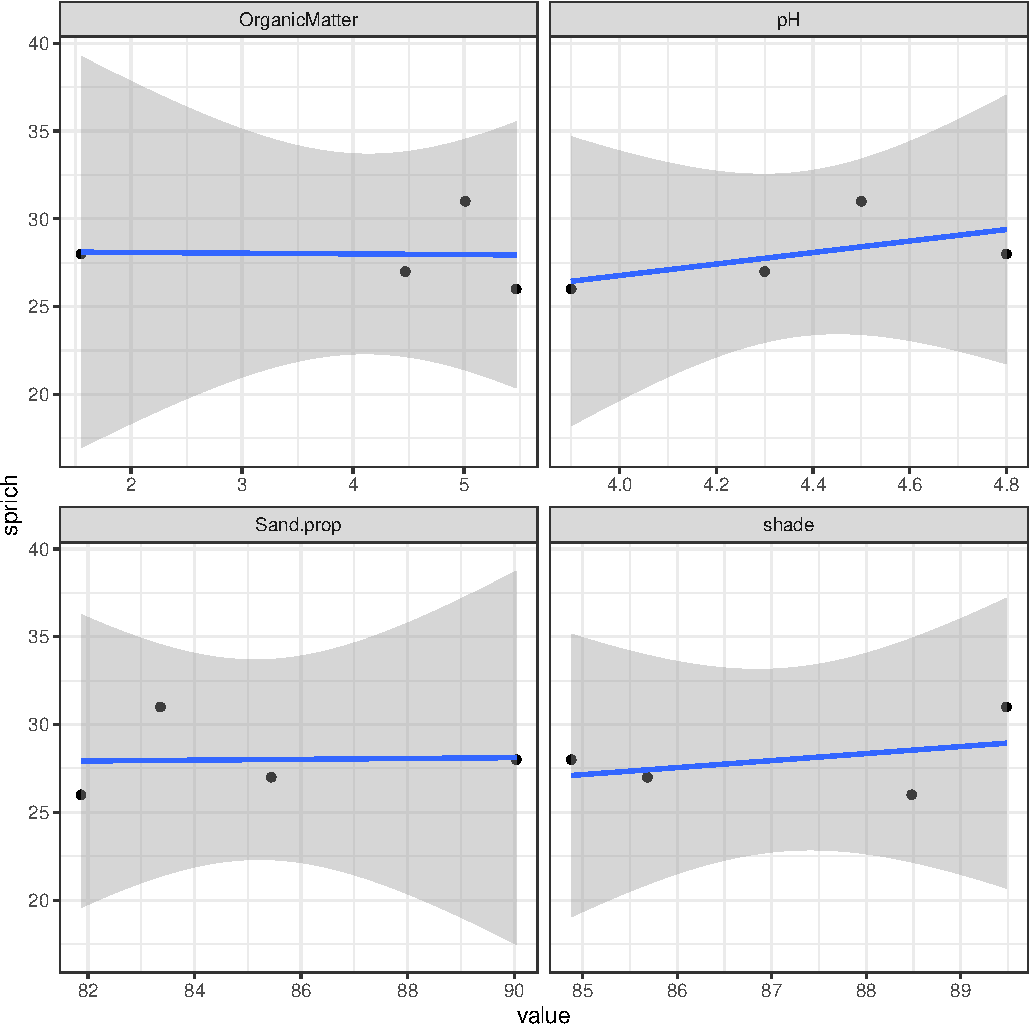
\includegraphics{ms_files/figure-pdf/fig-figName-1.pdf}

}

\caption{\label{fig-figName}\textbf{Figure caption here.} With more
caption text here.}

\end{figure}

Or if you already have the figure and want to cite it as
Fig.~\ref{fig-figByHand}.

\begin{figure}[H]

{\centering 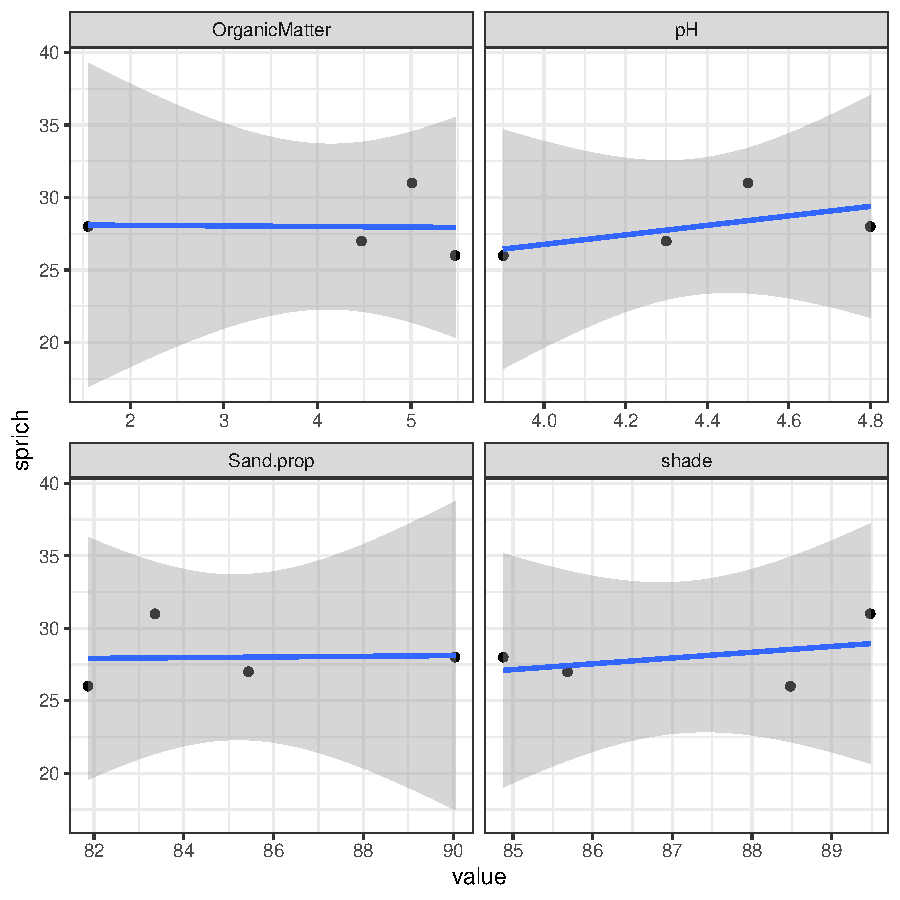
\includegraphics[width=0.7\textwidth,height=\textheight]{../Figs/plot.pdf}

}

\caption{\label{fig-figByHand}\textbf{Figure by hand caption here.} With
more caption text here.}

\end{figure}

Another example is Fig.~\ref{fig-figS1} in the Appendix.

More details can be found at
\href{https://quarto.org/docs/authoring/figures.html}{here}.

\hypertarget{references}{%
\section{References}\label{references}}

\hypertarget{refs}{}
\begin{CSLReferences}{1}{0}
\leavevmode\vadjust pre{\hypertarget{ref-adair_single-pool_2010}{}}%
Adair, E. C., S. E. Hobbie, and R. K. Hobbie. 2010.
\href{https://doi.org/10.1890/09-0430.1}{Single-pool exponential
decomposition models: Potential pitfalls in their use in ecological
studies}. Ecology 91:1225--1236.

\leavevmode\vadjust pre{\hypertarget{ref-clark_loss_2008}{}}%
Clark, C. M., and D. Tilman. 2008.
\href{https://doi.org/10.1038/nature06503}{Loss of plant species after
chronic low-level nitrogen deposition to prairie grasslands}. Nature
451:712--715.

\leavevmode\vadjust pre{\hypertarget{ref-eriksson_seed_1993}{}}%
Eriksson, O., and J. Ehrlén. 1993.
\href{http://dx.doi.org/10.1007/BF00317624}{Seed and microsite
limitation of recruitment in plant populations}. Oecologia 92:361--366.

\leavevmode\vadjust pre{\hypertarget{ref-williamson_dissolved_1999}{}}%
Williamson, C. E., D. P. Morris, M. L. Pace, and O. G. Olson. 1999.
Dissolved organic carbon and nutrients as regulators of lake ecosystems:
Resurrection of a more integrated paradigm. Limnology and Oceanography
44:795--803.

\end{CSLReferences}

\clearpage

\setcounter{page}{0}
\pagenumbering{arabic}
\setcounter{page}{1}

\setcounter{figure}{0}
\setcounter{table}{0}
\renewcommand {\thetable}{S\arabic{table}}
\renewcommand {\thefigure}{S\arabic{figure}}

\hypertarget{supporting-information}{%
\section{Supporting Information}\label{supporting-information}}

Some text here.

\hypertarget{figures-1}{%
\subsection{Figures}\label{figures-1}}

\begin{Shaded}
\begin{Highlighting}[]
\NormalTok{knitr}\SpecialCharTok{::}\FunctionTok{include\_graphics}\NormalTok{(}\AttributeTok{path =}\NormalTok{ here}\SpecialCharTok{::}\FunctionTok{here}\NormalTok{(}\StringTok{"Figs/plot.pdf"}\NormalTok{))}
\end{Highlighting}
\end{Shaded}

\begin{figure}[H]

{\centering 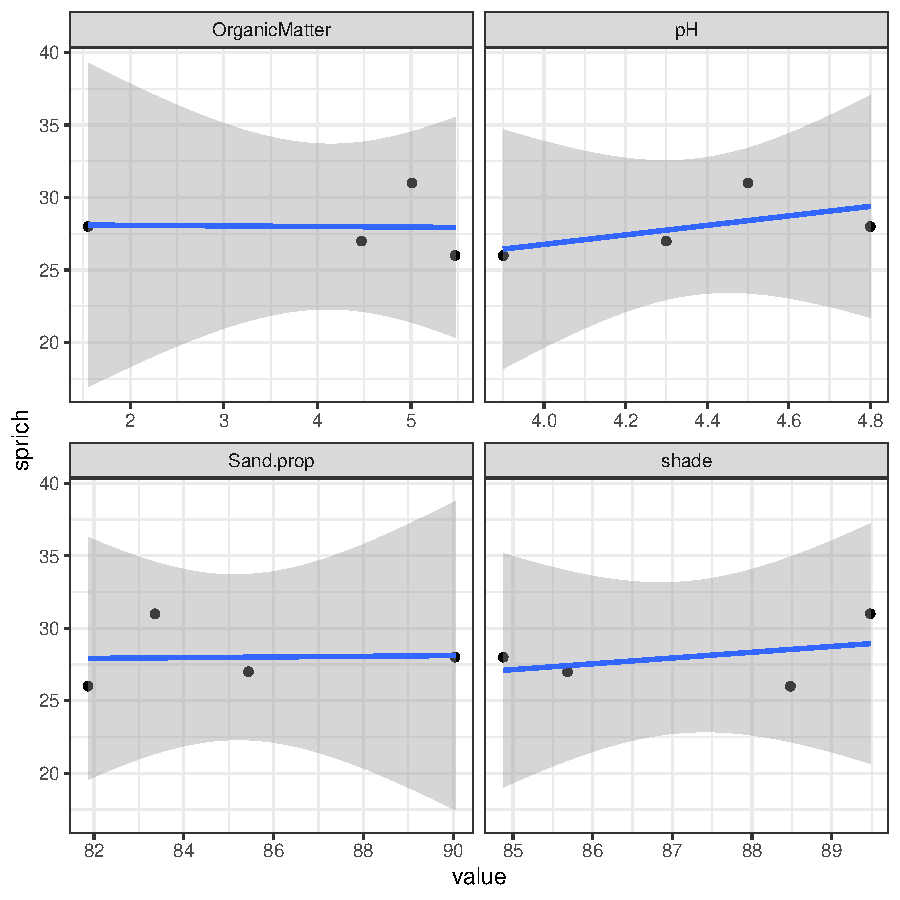
\includegraphics[width=0.7\textwidth,height=\textheight]{../Figs/plot.pdf}

}

\caption{\label{fig-figS1}\textbf{Figure caption here.} With more
caption text here.}

\end{figure}



\end{document}
